\documentclass[tikz,border=6mm]{standalone}

\begin{document}

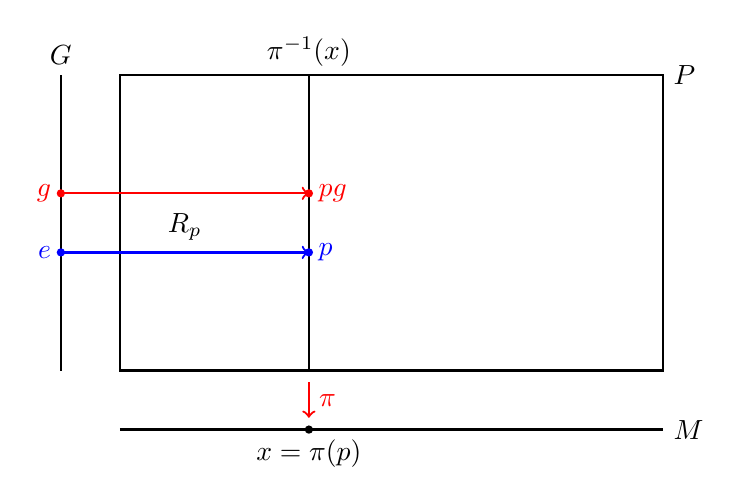
\begin{tikzpicture}[scale=1.5]

% Outer rectangle for the fiber bundle
  \draw[thick] (-2.3,0) rectangle (2.3,2.5) node[right] {$P$};
% Base manifold (M)
\draw[thick] (-2.3,-0.5) -- (2.3,-0.5) node[right] {$M$};
\draw[thick] (-2.8,0) -- (-2.8,2.5) node[above] {$G$};
% Highlight one tangent space TxM
\draw[thick] (-0.7,0) -- (-0.7,2.5);
\node at (-0.7,2.7) {$\pi^{-1}(x)$};
\fill[red] (-0.7,1.5) circle (1pt) node[right] {$pg$};
\fill[red] (-2.8,1.5) circle (1pt) node[left]{$g$};

\fill[blue] (-0.7,1) circle (1pt) node[right]{$p$};
\fill[blue] (-2.8,1) circle (1pt) node[left]{$e$};

\draw[red,->,thick](-2.8,1.5) -- (-0.7, 1.5) node[black,pos = 0.5,below,yshift = -3.5]{$R_p$};
\draw[blue,->,thick](-2.8,1) -- (-0.7, 1);
% Labels
\fill (-0.7,-0.5) circle (1pt);
\node[below] at (-0.7,-0.5) {$x = \pi(p)$};
% Projection arrow (pi)
\draw[red,->,thick] (-0.7,-0.1) -- (-0.7,-0.4) node[midway,right] {$\pi$};

\end{tikzpicture}

\end{document}


